\documentclass{article}
\usepackage[utf8]{inputenc}
\usepackage{graphicx}
\usepackage{caption}
\usepackage{subcaption}

\usepackage{float}

\begin{document}

\section{Resultados}

Resultados da avaliação com as métricas de paper de PRL.

\subsection{Plot \textbf{set\_ylim} = auto}
Os gráficos das imagens tem o axis Y, tem a faixa  em automático para os valores de FR e TVR. Lembrando que os valores de TF e TVR tem como máximo 1 e como mínimo 0

See the next images \ref{fig:tracklet_tau10}  \ref{fig:tracklet_tau100}  \ref{fig:tracklet_tau1000}

\begin{figure}[H]
    \begin{subfigure}{0.8\textwidth}
        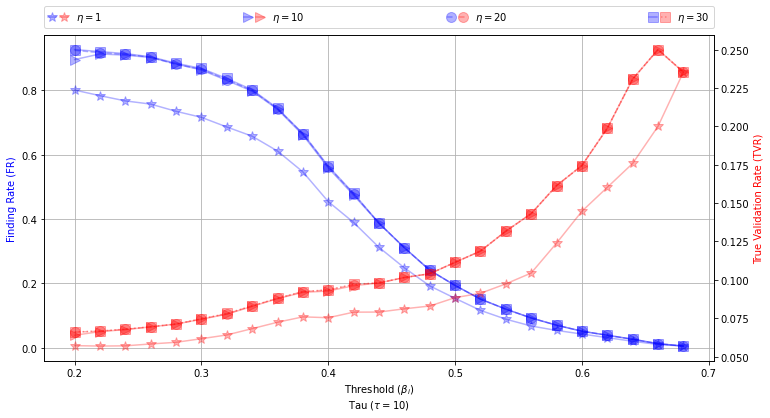
\includegraphics[width=11cm, height=6cm]{images_results/tracklet_tau10.png} 
        \caption{Tracklet methodology}
        \label{fig:subim1}
    \end{subfigure}
    
    \begin{subfigure}{0.9\textwidth}
        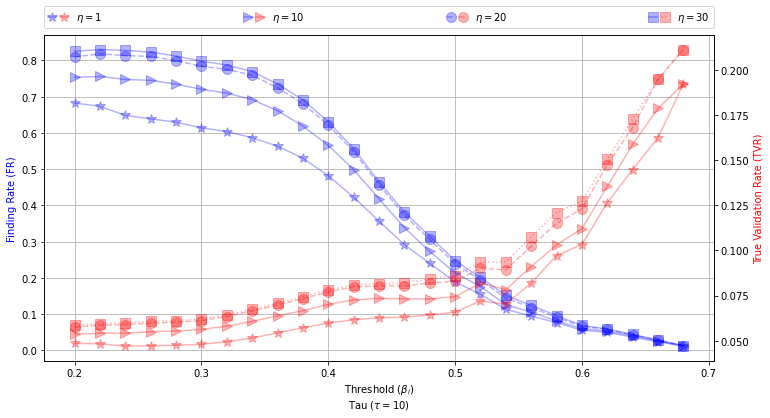
\includegraphics[width=11cm, height=6cm]{images_results/yolo_tau10.png}
        \caption{Yolo+REID-baseline methodology}
        \label{fig:subim2}
    \end{subfigure}

\caption{Results for $\tau = 10$}
\label{fig:tracklet_tau10}
\end{figure}


\begin{figure}[H]
    \begin{subfigure}{0.9\textwidth}
        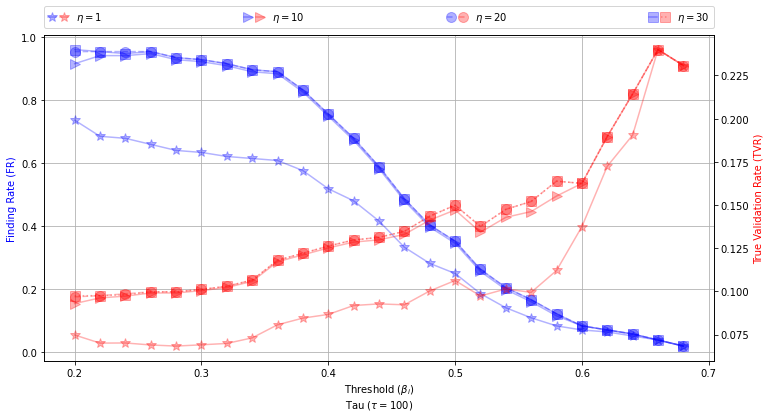
\includegraphics[width=12cm, height=7cm]{images_results/tracklet_tau100.png} 
        \caption{Tracklet methodology}
        \label{fig:subim1}
    \end{subfigure}
    
    \begin{subfigure}{0.9\textwidth}
        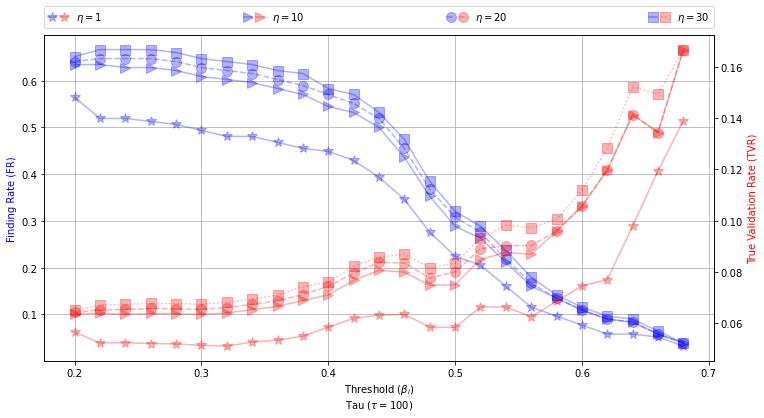
\includegraphics[width=12cm, height=7cm]{images_results/yolo_tau100.png}
        \caption{Yolo+REID-baseline methodology}
        \label{fig:subim2}
    \end{subfigure}

\caption{Results for $\tau = 100$}
\label{fig:tracklet_tau100}
\end{figure}


\begin{figure}[H]
    \begin{subfigure}{0.9\textwidth}
        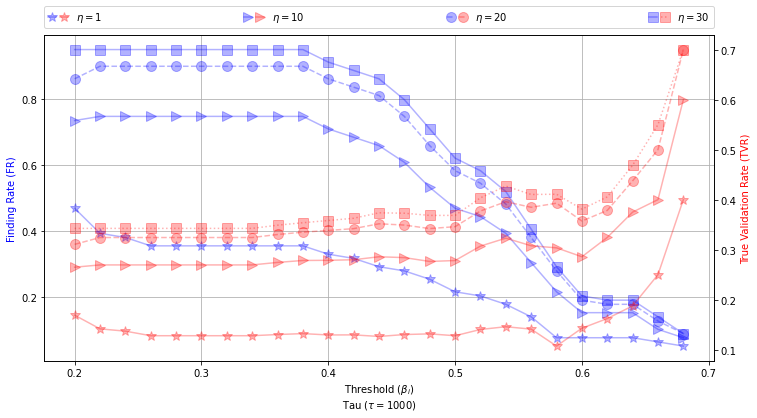
\includegraphics[width=12cm, height=7cm]{images_results/tracklet_tau1000.png} 
        \caption{Tracklet methodology}
        \label{fig:subim1}
    \end{subfigure}
    
    \begin{subfigure}{0.9\textwidth}
        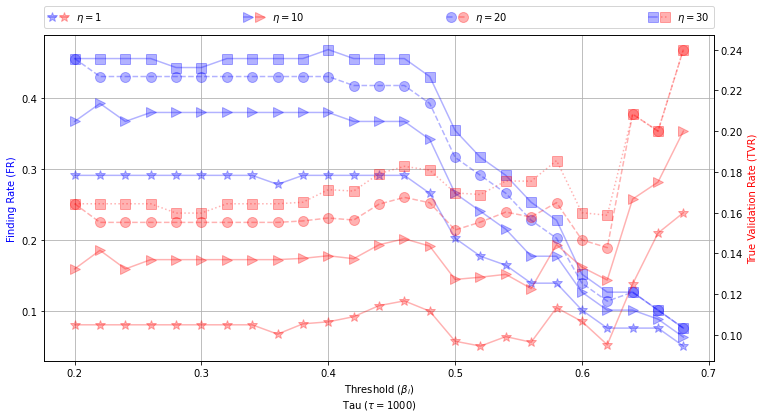
\includegraphics[width=12cm, height=7cm]{images_results/yolo_tau1000.png}
        \caption{Yolo+REID-baseline methodology}
        \label{fig:subim2}
    \end{subfigure}

\caption{Results for $\tau = 1000$}
\label{fig:tracklet_tau1000}
\end{figure}




\newpage
\newpage
\newpage


\subsection{Plot with \textbf{set\_ylim} = (0,1)  }  
Os gráficos das imagens tem o axis Y, tem a faixa  entre 0 e 1 para os valores de FR e TVR. Lembrando que os valores de TF e TVR tem como máximo 1 e como mínimo 0.

See the next images \ref{fig:tracklet_tau10_norm} \ref{fig:tracklet_tau100_norm} \ref{fig:tracklet_tau1000_norm}


\begin{figure}[H]
    \begin{subfigure}{0.9\textwidth}
        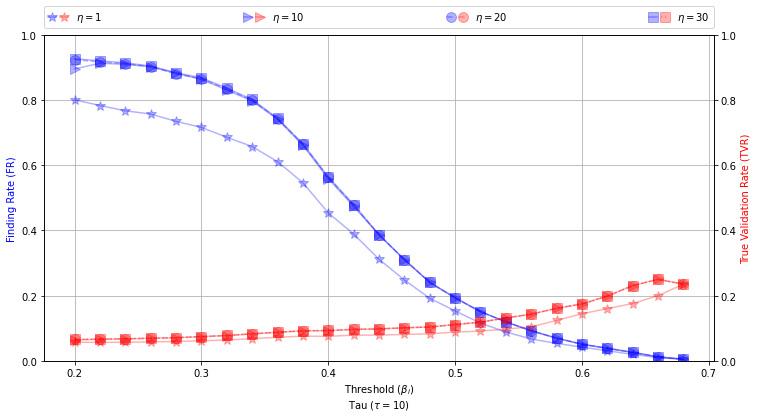
\includegraphics[width=12cm, height=7cm]{images_results/tracklet_tau10_norm.png} 
        \caption{Tracklet methodology}
        \label{fig:subim1}
    \end{subfigure}
    
    \begin{subfigure}{0.9\textwidth}
        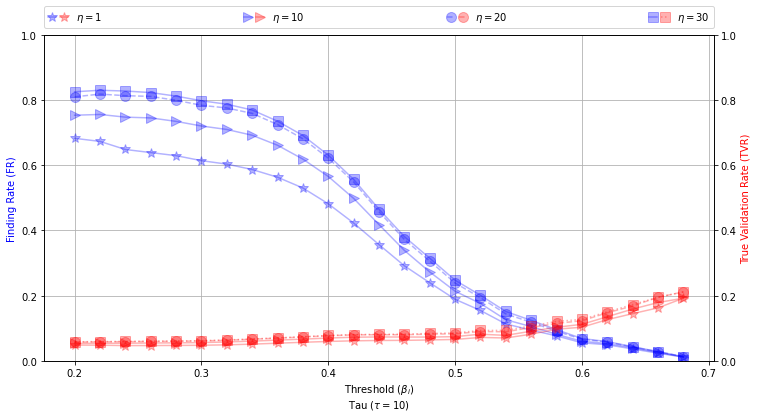
\includegraphics[width=12cm, height=7cm]{images_results/yolo_tau10_norm.png}
        \caption{Yolo+REID-baseline methodology}
        \label{fig:subim2}
    \end{subfigure}

\caption{Results for $\tau = 10$}
\label{fig:tracklet_tau10_norm}
\end{figure}


\begin{figure}[H]
    \begin{subfigure}{0.9\textwidth}
        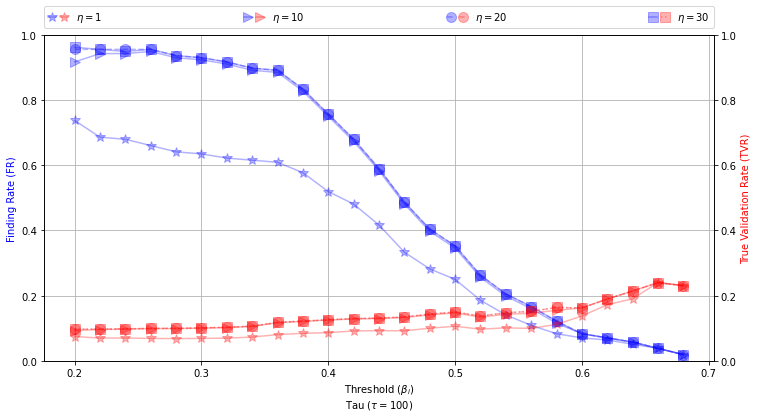
\includegraphics[width=12cm, height=7cm]{images_results/tracklet_tau100_norm.png} 
        \caption{Tracklet methodology}
        \label{fig:subim1}
    \end{subfigure}
    
    \begin{subfigure}{0.9\textwidth}
        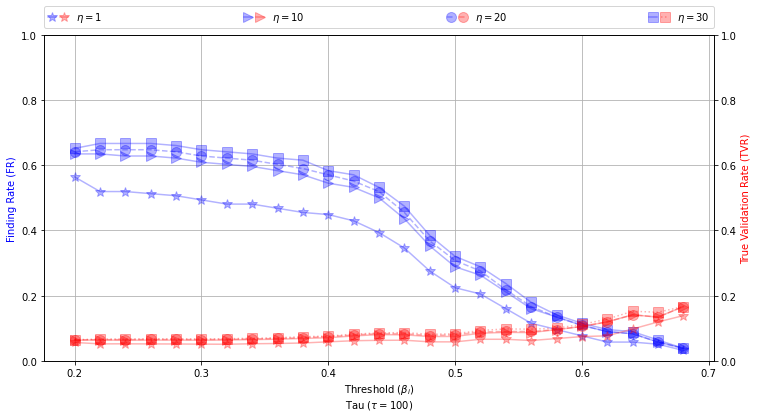
\includegraphics[width=12cm, height=7cm]{images_results/yolo_tau100_norm.png}
        \caption{Yolo+REID-baseline methodology}
        \label{fig:subim2}
    \end{subfigure}

\caption{Results for $\tau = 100$}
\label{fig:tracklet_tau100_norm}
\end{figure}


\begin{figure}[H]
    \begin{subfigure}{0.9\textwidth}
        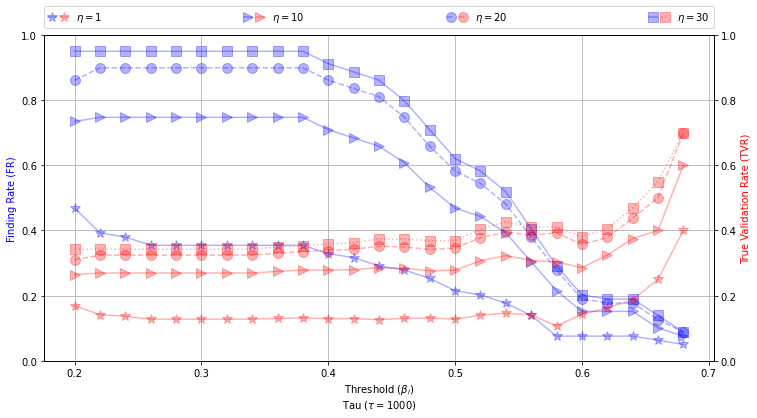
\includegraphics[width=12cm, height=7cm]{images_results/tracklet_tau1000_norm.png} 
        \caption{Tracklet methodology}
        \label{fig:subim1}
    \end{subfigure}
    
    \begin{subfigure}{0.9\textwidth}
        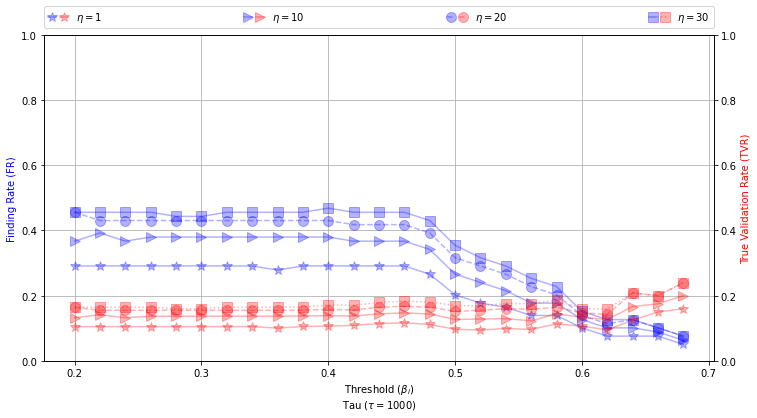
\includegraphics[width=12cm, height=7cm]{images_results/yolo_tau1000_norm.png}
        \caption{Yolo+REID-baseline methodology}
        \label{fig:subim2}
    \end{subfigure}

\caption{Results for $\tau = 1000$}
\label{fig:tracklet_tau1000_norm}
\end{figure}




\end{document}
